% La Grande Démission — Cover V3-13 Design System
% Compile with: xelatex design-system-lgd.tex
\documentclass[a4paper,11pt]{article}

\usepackage[margin=2.2cm]{geometry}
\usepackage{fontspec}
\usepackage[table]{xcolor}
\usepackage{tikz}
\usepackage{tcolorbox}
\usepackage{graphicx}
\usepackage{tabularx}
\usepackage{booktabs}
\usepackage{colortbl}
\usepackage{enumitem}
\usepackage[hidelinks]{hyperref}
\usepackage{fancyhdr}
\usepackage{parskip}
\usepackage{multicol}

\tcbuselibrary{skins,breakable}
\usetikzlibrary{shadows,shadings}
\usepackage{pifont}
\usepackage{titlesec}

% ─── Fonts ───
\setmainfont{Avenir Next}[
  UprightFont = * Regular,
  BoldFont = * Bold,
  ItalicFont = * Italic,
  BoldItalicFont = * Bold Italic,
]
\setsansfont{Avenir Next}
\setmonofont{Menlo}
% Knewave is the actual cover font (Google Fonts). Install it for accurate rendering.
% Fallback: Marker Felt (pre-installed macOS) — approximate only.
% To install: download from https://fonts.google.com/specimen/Knewave
% then double-click the .ttf to add it to Font Book.
\IfFontExistsTF{Knewave}{%
  \newcommand{\knewave}{\fontspec{Knewave}}%
}{%
  \newcommand{\knewave}{\fontspec{Marker Felt}\bfseries}%
}

% ─── Colors ───
\definecolor{lgdIndigo}{HTML}{2D1B69}
\definecolor{lgdViolet}{HTML}{7B3FE4}
\definecolor{lgdRed}{HTML}{FF4444}
\definecolor{lgdYellow}{HTML}{FFE135}
\definecolor{lgdLilas}{HTML}{C4B5FD}
\definecolor{lgdLavande}{HTML}{9B8EC4}
\definecolor{lgdTerracotta}{HTML}{C2704A}
\definecolor{lgdDark}{HTML}{1C1235}
\definecolor{lgdCream}{HTML}{FAE8D0}
\definecolor{lgdWarm}{HTML}{E8835C}
\definecolor{lgdGreen}{HTML}{00E5A0}
\definecolor{pageBg}{HTML}{FAFAF8}
\definecolor{cardBg}{HTML}{FFFFFF}
\definecolor{grayLight}{HTML}{F3F4F6}
\definecolor{grayMid}{HTML}{9CA3AF}
\definecolor{grayDark}{HTML}{4B5563}

\pagecolor{pageBg}

% ─── Table styling ───
\definecolor{tableHeader}{HTML}{F0F0F0}
\definecolor{tableRowAlt}{HTML}{F9FAFB}
\newcommand{\tableheader}{\rowcolor{tableHeader}\bfseries}

% ─── Section styling (after colors are defined) ───
\titleformat{\section}
  {\fontsize{22}{26}\selectfont\bfseries\sffamily\color{lgdIndigo}}
  {\thesection.}{0.5em}{}

\titleformat{\subsection}
  {\fontsize{14}{18}\selectfont\bfseries\sffamily\color{grayDark}}
  {\thesubsection}{0.5em}{}

% ─── Header/Footer ───
\pagestyle{fancy}
\fancyhf{}
\renewcommand{\headrulewidth}{0pt}
\fancyfoot[L]{\small\color{grayMid}La Grande Démission Design System — Denis Henin · uixbydenis.eu}
\fancyfoot[R]{\small\color{grayMid}\thepage}

% ─── Custom commands ───
\newcommand{\colorswatch}[3]{%
  \begin{tikzpicture}
    \fill[#1, rounded corners=4pt] (0,0) rectangle (1.2,1.2);
    \node[anchor=west, font=\small\bfseries, text=grayDark] at (1.45,0.75) {#2};
    \node[anchor=west, font=\footnotesize\ttfamily, text=grayMid] at (1.45,0.35) {#3};
  \end{tikzpicture}%
}

\newcommand{\tagpill}[2]{%
  \tikz[baseline=(tag.base)]{%
    \node[fill=#1, text=white, rounded corners=3pt, inner sep=3pt, font=\tiny\bfseries] (tag) {#2};%
  }%
}

\newcommand{\sectionrule}{%
  \vspace{4pt}%
  \noindent
\begin{tikzpicture}
    \shade[left color=lgdIndigo, right color=lgdRed] (0,0) rectangle (\textwidth, 2.5pt);
  \end{tikzpicture}%
  \vspace{6pt}%
}

% ─── tcolorbox styles ───
\tcbset{
  card/.style={
    enhanced,
    colback=cardBg,
    colframe=grayLight,
    boxrule=0.4pt,
    arc=6pt,
    left=12pt, right=12pt, top=10pt, bottom=10pt,
    fonttitle=\bfseries\sffamily,
    coltitle=grayDark,
    drop shadow={shadow xshift=0.5pt, shadow yshift=-1.5pt, opacity=0.12},
    breakable,
  },
  highlight card/.style={
    card,
    borderline north={2pt}{0pt}{lgdViolet!70!lgdIndigo},
  }
}

% ─── Do/Don't helpers ───
\newcommand{\doitem}[1]{\item[\color{lgdGreen}\ding{51}] #1}
\newcommand{\dontitem}[1]{\item[\color{lgdRed}\ding{55}] #1}

\begin{document}

% ═══════════════════════════════════════════
% TITLE PAGE
% ═══════════════════════════════════════════

\thispagestyle{empty}

\begin{tikzpicture}[remember picture, overlay]
  \shade[left color=lgdIndigo, right color=lgdRed]
    (current page.north west) rectangle ([yshift=-9cm]current page.north east);
  \fill[lgdDark]
    ([yshift=-9cm]current page.north west) rectangle (current page.south east);
\end{tikzpicture}

\vspace*{0.8cm}

\begin{center}
  
\includegraphics[width=9cm]{../covers/layers/cover-v3-13-text.png}\\[6pt]
  {\Large\color{white}\bfseries Cover V3-13 — Design System}\\[4pt]
  {\small\color{white!60}Version 1.0 — Mars 2026}\\[2pt]
  {\small\color{white!40}Denis Henin — Graphiste Designer @ bleen}
\end{center}

\vspace{0.4cm}

\begin{center}
  \begin{tikzpicture}
    \node[drop shadow={shadow xshift=1pt, shadow yshift=-2pt, opacity=0.3, fill=black}, inner sep=0pt] {%
      \includegraphics[width=7.5cm]{../covers/cover-v3-13.png}%
    };
  \end{tikzpicture}
\end{center}

\vfill

\begin{center}
  {\footnotesize\color{white!30}Cover « Rebond Indigo » · V3-13 · 3000×3000px}
\end{center}

\newpage

% ═══════════════════════════════════════════
% TABLE OF CONTENTS
% ═══════════════════════════════════════════

\tableofcontents
\newpage

% ═══════════════════════════════════════════
% 1. CONTEXTE
% ═══════════════════════════════════════════

\section{Contexte du podcast}
\sectionrule

\begin{tcolorbox}[card]
\rowcolors{2}{white}{tableRowAlt}
\begin{tabularx}{\textwidth}{@{}lX@{}}
\toprule
\tableheader Élément & Détail \\
\midrule
Nom & La Grande Démission \\
Tagline & « Quitter pour mieux rebondir » \\
Concept & Podcast qui explore le phénomène de la Grande Démission — pourquoi on part, ce qu'on trouve après \\
Producteur & bleen \\
Format & Épisodes thématiques, interviews et témoignages \\
Ton & Énergique, libérateur, punk sans être agressif \\
Audience & Actifs en reconversion, 25--45 ans, milieu urbain \\
Thèmes & Travail, sens, reconversion, burn-out, nouvelles formes d'emploi \\
Univers visuel & Contrastes vifs, palette indigo/violet/rouge, énergie punk \\
\bottomrule
\end{tabularx}
\end{tcolorbox}

\subsection{Positionnement}

Un podcast sur la transformation du rapport au travail. Le ton est \textbf{énergique et libérateur} — l'acte de démissionner n'est pas une fin mais un rebond. L'imagerie traduit cette énergie : papiers qui volent, bras levés, couleurs vives qui claquent.

\subsection{Identité visuelle V3-13 « Rebond »}

La version V3-13 est la palette « Rebond » — une direction visuelle construite sur le contraste maximal. Indigo électrique + jaune solaire = impossible à rater en miniature. Le personnage jette ses papiers en l'air, symbole de libération.

\subsection{Ce que la marque est}

\begin{itemize}[nosep]
  \item Énergique, libératrice, punk dans l'esprit
  \item Le rebond après la claque — pas la plainte
  \item Contrastes forts, couleurs qui claquent
  \item Accessible et directe, jamais moralisatrice
  \item Optimiste sur la transformation du travail
\end{itemize}

\subsection{Ce que la marque n'est pas}

\begin{itemize}[nosep]
  \item Victimaire ou défaitiste
  \item Corporate / RH / institutionnel
  \item Pastel ou feutrée
  \item Moralisatrice ou culpabilisante
  \item Froide ou distante
\end{itemize}

\newpage

% ═══════════════════════════════════════════
% 2. PALETTE DE COULEURS
% ═══════════════════════════════════════════

\section{Palette de couleurs}
\sectionrule

\subsection{Gradient de fond}

Le fond utilise un \textbf{dégradé diagonal} (135°) en trois étapes : indigo profond → violet électrique → rouge vif.

\begin{tcolorbox}[card]
\begin{center}
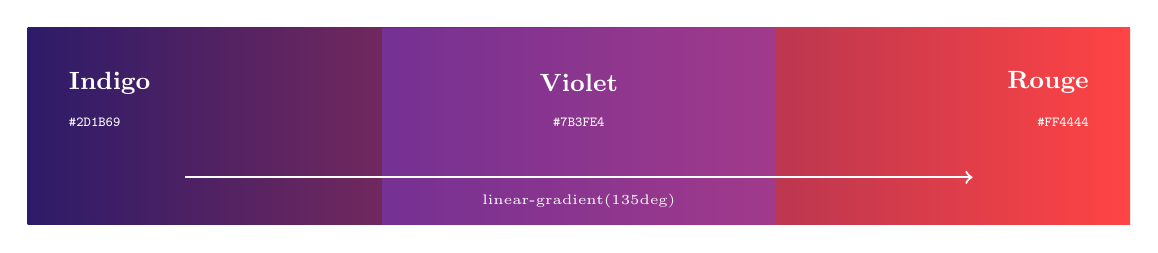
\begin{tikzpicture}
  \shade[left color=lgdIndigo, right color=lgdRed] (0,0) rectangle (14,2.5);
  \fill[lgdViolet, opacity=0.4] (4.5,0) rectangle (9.5,2.5);
  \node[font=\small\bfseries, text=white, anchor=west] at (0.4, 1.8) {Indigo};
  \node[font=\tiny\ttfamily, text=white, anchor=west] at (0.4, 1.3) {\#2D1B69};
  \node[font=\small\bfseries, text=white] at (7, 1.8) {Violet};
  \node[font=\tiny\ttfamily, text=white] at (7, 1.3) {\#7B3FE4};
  \node[font=\small\bfseries, text=white, anchor=east] at (13.6, 1.8) {Rouge};
  \node[font=\tiny\ttfamily, text=white, anchor=east] at (13.6, 1.3) {\#FF4444};
  \draw[white, thick, ->] (2, 0.6) -- (12, 0.6);
  \node[font=\tiny, text=white] at (7, 0.3) {linear-gradient(135deg)};
\end{tikzpicture}
\end{center}
\end{tcolorbox}

\begin{tcolorbox}[colback=grayLight!30, colframe=grayLight, boxrule=0.3pt, arc=3pt, left=8pt, right=8pt, top=4pt, bottom=4pt]
{\small\ttfamily CSS: background: linear-gradient(135deg, \#2D1B69, \#7B3FE4, \#FF4444);}
\end{tcolorbox}

\subsection{Couleurs principales}

\noindent
\colorswatch{lgdIndigo}{Indigo}{\#2D1B69}\hspace{18pt}%
\colorswatch{lgdViolet}{Violet}{\#7B3FE4}\hspace{18pt}%
\colorswatch{lgdRed}{Rouge}{\#FF4444}

\vspace{6pt}\noindent
\colorswatch{lgdYellow}{Jaune solaire}{\#FFE135}\hspace{18pt}%
\colorswatch{lgdLilas}{Lilas}{\#C4B5FD}

\subsection{Couleurs secondaires (palette Bleen/LGD)}

\noindent
\colorswatch{lgdLavande}{Lavande}{\#9B8EC4}\hspace{18pt}%
\colorswatch{lgdTerracotta}{Terracotta}{\#C2704A}\hspace{18pt}%
\colorswatch{lgdDark}{Dark}{\#1C1235}

\vspace{6pt}\noindent
\colorswatch{lgdCream}{Crème}{\#FAE8D0}\hspace{18pt}%
\colorswatch{lgdWarm}{Warm}{\#E8835C}

\subsection{Rôles des couleurs sur la cover V3-13}

\begin{tcolorbox}[card]
\begin{tabularx}{\textwidth}{@{}llX@{}}
\toprule
\textbf{Couleur} & \textbf{Hex} & \textbf{Usage sur la cover} \\
\midrule
Indigo & \texttt{\#2D1B69} & Fond haut-gauche, ancrage sombre \\
Violet & \texttt{\#7B3FE4} & Zone centrale du gradient, énergie \\
Rouge & \texttt{\#FF4444} & Fond bas-droite, tension/action \\
Blanc & \texttt{\#FFFFFF} & Texte « La Grande » — contraste max sur fond violet \\
Jaune solaire & \texttt{\#FFE135} & Texte « Démission » — impact visuel, énergie \\
Blanc 60\% & \texttt{rgba(255,255,255,0.6)} & Logo Bleen — discret \\
\bottomrule
\end{tabularx}
\end{tcolorbox}

\subsection{Contraste et lisibilité}

\begin{tcolorbox}[card, colframe=lgdYellow!50, title={\color{lgdIndigo}Choix de contraste}]
\begin{itemize}[nosep]
  \item \textbf{« La Grande » en blanc} plutôt qu'en jaune — le blanc offre un meilleur contraste sur la zone violet foncé du gradient
  \item \textbf{« Démission » en jaune solaire} — le jaune \texttt{\#FFE135} claque fort sur le violet/rouge. C'est le mot-clé, il doit dominer visuellement
  \item Le lilas \texttt{\#C4B5FD} (version initiale) manquait de punch sur le fond — remplacé par le jaune
\end{itemize}
\end{tcolorbox}

% ═══════════════════════════════════════════
% 3. TYPOGRAPHIE
% ═══════════════════════════════════════════

\section{Typographie}
\sectionrule

\subsection{Hiérarchie typographique}

\begin{tcolorbox}[card]
\rowcolors{2}{white}{tableRowAlt}
\begin{tabularx}{\textwidth}{@{}llXl@{}}
\toprule
\tableheader Usage & Police & Justification & Taille \\
\midrule
Titre cover & Knewave & Énergie, caractère punk & 430--580px (export 3k) \\
Sous-titres & Plus Jakarta Sans Bold & Lisibilité, modernité & 24--32pt \\
Corps & Plus Jakarta Sans Regular & Neutralité, confort & 14--18pt \\
Accents & Caveat, Patrick Hand & Rappel du côté manuscrit & variable \\
\bottomrule
\end{tabularx}
\end{tcolorbox}

\newpage

\subsection{Titre « La Grande Démission »}

\begin{tcolorbox}[card]
\begin{center}
\includegraphics[width=0.75\linewidth]{../covers/cover-v3-13.png}
\end{center}

\vspace{6pt}

\rowcolors{2}{white}{tableRowAlt}
\begin{tabularx}{\textwidth}{@{}lX@{}}
\toprule
\tableheader Propriété & Valeur \\
\midrule
Police & Knewave (Google Fonts) \\
« La Grande » & Blanc \texttt{\#FFFFFF}, 430px (export 3k), 50px max (preview) \\
« Démission » & Jaune \texttt{\#FFE135}, 580px (export 3k), 68px max (preview) \\
Stroke & Contour noir semi-transparent (14--18px à l'échelle 3000px) \\
Paint-order & \texttt{stroke fill} — contour sous le remplissage \\
Ombres & 4 ombres directionnelles + glow diffus \\
Position & \texttt{top:6\%}, centré horizontalement \\
\bottomrule
\end{tabularx}
\end{tcolorbox}

\subsection{Traitement du texte sur la cover}

Le titre est traité avec plusieurs couches d'effets pour assurer la lisibilité sur le gradient :

\begin{enumerate}[nosep]
  \item \textbf{Remplissage} : blanc pur \texttt{\#FFFFFF} (« La Grande ») / jaune \texttt{\#FFE135} (« Démission »)
  \item \textbf{Contour (stroke)} : noir à 60--70\% d'opacité, 14--18px d'épaisseur (à l'échelle 3000px)
  \item \textbf{Paint-order} : \texttt{stroke fill} — le contour est peint sous le remplissage
  \item \textbf{Ombres} : 4 ombres directionnelles + 1 ombre douce (glow diffus)
  \item \textbf{Ratio de taille} : « Démission » $\sim$35\% plus grand que « La Grande » (ratio 1:1.35)
\end{enumerate}

\newpage

% ═══════════════════════════════════════════
% 4. ILLUSTRATION
% ═══════════════════════════════════════════

\section{Illustration}
\vspace{-6pt}
\sectionrule

\subsection{Style}

\begin{tcolorbox}[card]
\begin{tabularx}{\textwidth}{@{}lX@{}}
\toprule
\textbf{Propriété} & \textbf{Description} \\
\midrule
Type & Illustration vectorielle flat design \\
Rendu & Semi-réaliste, stylisé \\
Palette perso & Costume bleu marine, chemise blanche, peau tons chauds \\
Émotion & Joie, libération, énergie — bras levés, bouche ouverte \\
Éléments & Papiers qui volent (symbole de démission) \\
Perspective & Vue de face, légère contre-plongée \\
\bottomrule
\end{tabularx}
\end{tcolorbox}

\subsection{Personnage}

\begin{itemize}[nosep]
  \item Homme en costume bleu marine, bras levés en V
  \item Expression de joie/libération — bouche grande ouverte, rire
  \item Papiers blancs qui volent autour de lui (lettres de démission)
  \item Le personnage occupe la moitié inférieure de la cover
\end{itemize}

\subsection{Traitement de l'image}

\begin{tcolorbox}[card]
\begin{tabularx}{\textwidth}{@{}lX@{}}
\toprule
\textbf{Fichier} & \textbf{Détail} \\
\midrule
Source originale & \texttt{test\_1.png} (1028 × 932 px, RGBA) \\
En production & \texttt{test\_1\_clean.png} — feuille en bas à droite retirée \\
Placement & \texttt{width:90\%; left:5\%; bottom:-12\%} \\
Filtre & Glow violet \texttt{rgba(123,63,228,0.4)} + drop-shadow noir \\
\bottomrule
\end{tabularx}
\end{tcolorbox}

\subsection{Nettoyage de l'image}

La feuille de papier en bas à droite (cluster \#73, 6034 pixels) a été retirée de l'image originale pour dégager la zone du logo Bleen. L'opération a été faite par détection de clusters de pixels clairs ($>$160 RGB) + mise en transparence. L'image originale \texttt{test\_1.png} est conservée intacte.

\newpage

% ═══════════════════════════════════════════
% 5. COMPOSITION
% ═══════════════════════════════════════════

\section{Composition \& mise en page}
\sectionrule

\subsection{Structure de la cover (3000×3000px)}

\begin{tcolorbox}[card]
\begin{center}
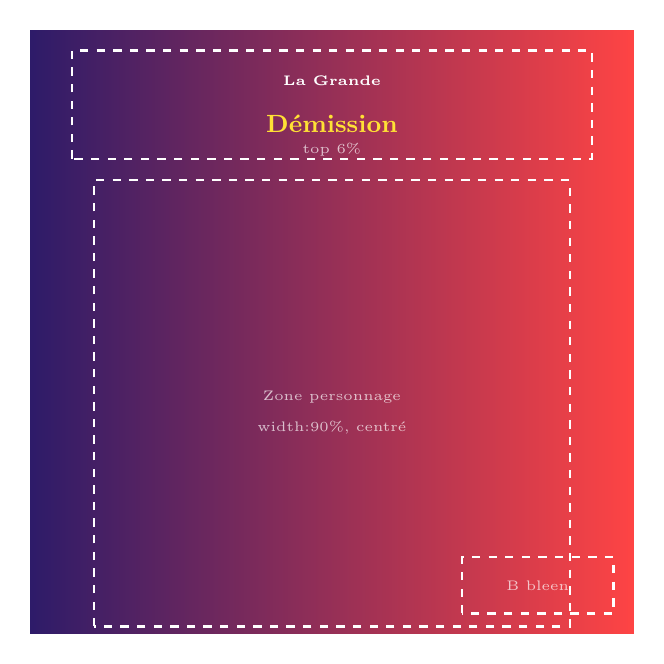
\begin{tikzpicture}[scale=0.55]
  \shade[left color=lgdIndigo, right color=lgdRed] (0,0) rectangle (14,14);
  \draw[white, thick] (0,0) rectangle (14,14);

  % Title zone
  \draw[white, dashed, thick] (1,11) rectangle (13,13.5);
  \node[font=\tiny\bfseries, text=white] at (7,12.8) {La Grande};
  \node[font=\small\bfseries, text=lgdYellow] at (7,11.8) {Démission};
  \node[font=\tiny, text=white, opacity=0.7] at (7,11.2) {top 6\%};

  % Character zone
  \draw[white, dashed, thick] (1.5,0.2) rectangle (12.5,10.5);
  \node[font=\tiny, text=white, opacity=0.7] at (7,5.5) {Zone personnage};
  \node[font=\tiny, text=white, opacity=0.7] at (7,4.8) {width:90\%, centré};

  % Logo zone
  \draw[white, dashed, thick] (10,0.5) rectangle (13.5,1.8);
  \node[font=\tiny, text=white, opacity=0.7] at (11.75,1.15) {B bleen};
\end{tikzpicture}
\end{center}
\end{tcolorbox}

\subsection{Règles de composition}

\begin{itemize}[nosep]
  \item \textbf{Titre en haut} : toujours au-dessus du personnage, jamais derrière
  \item \textbf{Personnage centré} : point focal, expression de libération
  \item \textbf{Fond gradient} : pas de photo, pas de paysage — le gradient indigo/rouge suffit
  \item \textbf{Papiers qui volent} : renforcent la dynamique, ne doivent pas couvrir le titre
  \item \textbf{Logo} : B bleen regroupés, discret, bas-droite
\end{itemize}

\subsection{Calques d'export}

Chaque cover est exportée en calques séparés (3000×3000px PNG) :

\begin{tcolorbox}[card]
\rowcolors{2}{white}{tableRowAlt}
\begin{tabularx}{\textwidth}{@{}llXl@{}}
\toprule
\tableheader Calque & Fichier & Contenu & Taille \\
\midrule
Background & \texttt{cover-v3-13-bg.png} & Gradient + vignette & 4.9 MB \\
Personnage & \texttt{cover-v3-13-character.png} & Illustration, fond transparent & 2.9 MB \\
Texte & \texttt{cover-v3-13-text.png} & Titre, fond transparent & 674 KB \\
Logo & \texttt{cover-v3-13-logo.png} & B bleen, fond transparent & 66 KB \\
\midrule
Composite & \texttt{cover-v3-13.png} & Tous calques fusionnés & 6.1 MB \\
\bottomrule
\end{tabularx}
\end{tcolorbox}

\newpage

% ═══════════════════════════════════════════
% 6. LOGO BLEEN
% ═══════════════════════════════════════════

\section{Logo Bleen}
\sectionrule

\subsection{Composition du bloc logo}

Le logo sur la cover combine deux éléments SVG en un seul bloc :

\begin{tcolorbox}[card]
\rowcolors{2}{white}{tableRowAlt}
\begin{tabularx}{\textwidth}{@{}lX@{}}
\toprule
\tableheader Élément & Détail \\
\midrule
Icône « B » & Forme double-bulle Bleen, viewBox 0 0 200 280 \\
Texte « bleen » & Logotype, viewBox 270 60 450 160 \\
Couleur & \texttt{rgba(255,255,255,0.6)} — blanc à 60\% d'opacité \\
Gap & 18px entre icône et texte (à l'échelle 3000px) \\
Position & \texttt{bottom:6\%; right:6\%} (bas-droite) \\
Filtre & \texttt{drop-shadow(0 4px 8px rgba(0,0,0,0.2))} \\
\bottomrule
\end{tabularx}
\end{tcolorbox}

\subsection{Ratios du logo SVG (source : bleenconsulting.webflow.io)}

Proportions extraites du SVG officiel Bleen (viewBox \texttt{0 0 720 280}) :

\begin{tcolorbox}[card]
\rowcolors{2}{white}{tableRowAlt}
\begin{tabularx}{\textwidth}{@{}lX@{}}
\toprule
\tableheader Mesure & Valeur \\
\midrule
ViewBox global & 720 $\times$ 280 (ratio 18:7 $\approx$ 2.57:1) \\
\midrule
\multicolumn{2}{@{}l}{\textit{Symbole « B »}} \\
Bounding box & x=0$\rightarrow$200, y=0$\rightarrow$280 — soit 200 $\times$ 280 (ratio 5:7) \\
Grand cercle & 200 $\times$ 200 (y=80$\rightarrow$280) \\
Petit cercle & 160 $\times$ 160 (y=0$\rightarrow$160) — ratio petit/grand = 4:5 \\
Chevauchement & 80 unités verticales (y=80$\rightarrow$160) \\
\midrule
\multicolumn{2}{@{}l}{\textit{Texte « bleen »}} \\
Bounding box & x=270$\rightarrow$720, y=70$\rightarrow$210 — soit 450 $\times$ 140 \\
\midrule
\multicolumn{2}{@{}l}{\textit{Rapports clés}} \\
Symbole : Gap : Texte (largeur) & 200 : 70 : 450 ($\approx$ 28\% : 10\% : 62\%) \\
Largeur symbole / largeur texte & 200/450 = 0.444 (le symbole fait 44\% du texte) \\
Hauteur symbole / hauteur texte & 280/140 = 2.0 (le symbole fait 2$\times$ la hauteur du texte) \\
\bottomrule
\end{tabularx}
\end{tcolorbox}

\subsection{Règles}

\begin{itemize}[nosep]
  \item Opacité réduite pour ne pas détourner l'attention du personnage
  \item Ombre légère pour la lisibilité sur fonds clairs et sombres
\end{itemize}

% ═══════════════════════════════════════════
% 7. EFFETS & OVERLAYS
% ═══════════════════════════════════════════

\newpage

\section{Effets \& overlays}
\sectionrule

La cover V3-13 utilise plusieurs couches d'effets pour renforcer la profondeur et l'impact visuel. Plus chargée que Velotaf, elle joue sur les vignettes et le glow violet pour créer une ambiance « punk électrique ».

\begin{tcolorbox}[card]
\begin{tabularx}{\textwidth}{@{}llX@{}}
\toprule
\textbf{Effet} & \textbf{Intensité} & \textbf{Description} \\
\midrule
Vignette & 18\% top, 12\% bottom & Assombrissement léger haut et bas du gradient \\
Vignette radiale & 15\% bords & Assombrissement elliptique des bords \\
Grain & 3.5\% opacité & Texture de bruit fractal, blend mode overlay \\
Glow personnage & Violet & \texttt{drop-shadow rgba(123,63,228,0.4)} — halo violet autour du personnage \\
Drop-shadow & Noir & \texttt{0 12px 24px rgba(0,0,0,0.4)} + \texttt{0 48px 96px rgba(0,0,0,0.15)} \\
Text stroke & 14--18px & Contour noir à 60--70\% autour des titres \\
Text shadow & Multi & 4 directions + glow diffus \\
\bottomrule
\end{tabularx}
\end{tcolorbox}

% ═══════════════════════════════════════════
% 8. SPECS TECHNIQUES
% ═══════════════════════════════════════════

\newpage

\section{Spécifications techniques}
\sectionrule

\subsection{Format de la cover}

\begin{tcolorbox}[card]
\begin{tabularx}{\textwidth}{@{}lX@{}}
\toprule
\textbf{Propriété} & \textbf{Valeur} \\
\midrule
Dimensions & 3000 × 3000 px (carré) \\
Résolution & 72 DPI (optimisé écran) \\
Format & PNG 24-bit avec alpha (calques) / PNG opaque (composite) \\
Espace colorimétrique & sRGB \\
Poids composite & $\sim$6.1 MB \\
\bottomrule
\end{tabularx}
\end{tcolorbox}

\subsection{CSS de référence}

\begin{tcolorbox}[card, colback=lgdDark, coltext=white!90]
\begin{verbatim}
/* Gradient de fond */
background: linear-gradient(135deg, #2D1B69, #7B3FE4, #FF4444);

/* Vignette */
background: linear-gradient(to bottom,
  rgba(0,0,0,0.18) 0%, rgba(0,0,0,0.05) 40%,
  transparent 60%, rgba(0,0,0,0.12) 100%),
  radial-gradient(ellipse 80% 80% at 50% 40%,
  transparent 40%, rgba(0,0,0,0.15) 100%);

/* Personnage */
width: 90%; left: 5%; bottom: -12%;
filter: drop-shadow(0 0 3px rgba(123,63,228,0.4))
        drop-shadow(0 12px 24px rgba(0,0,0,0.4));

/* Titre "La Grande" */
font-family: 'Knewave', cursive;
font-size: 430px;  /* @ 3000px */
color: #FFFFFF;

/* Titre "Démission" */
font-size: 580px;  /* @ 3000px */
color: #FFE135;

/* Logo B bleen */
bottom: 6%; right: 6%;
color: rgba(255,255,255,0.6);
\end{verbatim}
\end{tcolorbox}

\newpage

% ═══════════════════════════════════════════
% 9. DÉCLINAISONS
% ═══════════════════════════════════════════

\section{Déclinaisons recommandées}
\sectionrule

\subsection{Formats réseaux sociaux}

\begin{tcolorbox}[card]
\rowcolors{2}{white}{tableRowAlt}
\begin{tabularx}{\textwidth}{@{}llX@{}}
\toprule
\tableheader Plateforme & Dimensions & Adaptation \\
\midrule
Instagram post & 1080 × 1080 & Cover art ou variante avec citation \\
Instagram story & 1080 × 1920 & Gradient vertical, personnage en bas \\
Bannière Twitter/X & 1500 × 500 & Personnage à gauche, titre à droite \\
Bannière LinkedIn & 1584 × 396 & Idem Twitter, adapté au format \\
Miniature YouTube & 1280 × 720 & Personnage + titre épisode en gros \\
\bottomrule
\end{tabularx}
\end{tcolorbox}

\subsection{Do's \& Don'ts}

\begin{multicols}{2}
\begin{tcolorbox}[card, title={\color{lgdGreen!80!black}Do's}, colframe=lgdGreen!30, borderline north={2pt}{0pt}{lgdGreen}]
\begin{itemize}[nosep, leftmargin=16pt]
  \doitem{Gradient indigo → rouge comme base}
  \doitem{Titre jaune solaire pour « Démission »}
  \doitem{Personnage avec papiers qui volent}
  \doitem{Contraste maximal pour lisibilité mobile}
  \doitem{Garder l'énergie punk/libération}
\end{itemize}
\end{tcolorbox}

\begin{tcolorbox}[card, title={\color{lgdRed}Don'ts}, colframe=lgdRed!30, borderline north={2pt}{0pt}{lgdRed}]
\begin{itemize}[nosep, leftmargin=16pt]
  \dontitem{Couleurs ternes ou pastels}
  \dontitem{Texte lilas sur fond violet (contraste faible)}
  \dontitem{Photos en fond}
  \dontitem{Ton corporate/sage}
  \dontitem{Surcharger avec trop d'éléments}
  \dontitem{Noir pur \texttt{\#000000}}
\end{itemize}
\end{tcolorbox}
\end{multicols}

\vfill

\begin{center}

\begin{tikzpicture}
  \shade[left color=lgdIndigo, right color=lgdRed] (0,0) rectangle (\textwidth, 2pt);
\end{tikzpicture}\\[8pt]
{\small\color{grayMid} Document généré le \today\ — Bleen Consulting}
\end{center}

\end{document}
